\section{The Power Transition}
Building on the work of Edward Carr (1939, 1945) and Organski (1958) constructed what was perhaps the first challenge to realism that was neither idealistic nor normative.

\begin{itemize}
    \item The international system is not anarchic.
    \item There is only one dominant state at any given time.
    \item Rather than wishing to maximize security or power, nations are interested in maximizing their \textbf{control over the rules and customs that govern international interactions} so that they can define the status quo according to their interests.
\end{itemize}

Bretton Woods Agreement $\Rightarrow$ These agreements still maintain a rule-based and normative influence on the trading practices of their members.

\textbf{Dissatisfaction} $\Rightarrow$ it is the more powerful dissatisfied states that represent the biggest threat to international peace and stability.

\begin{center}
    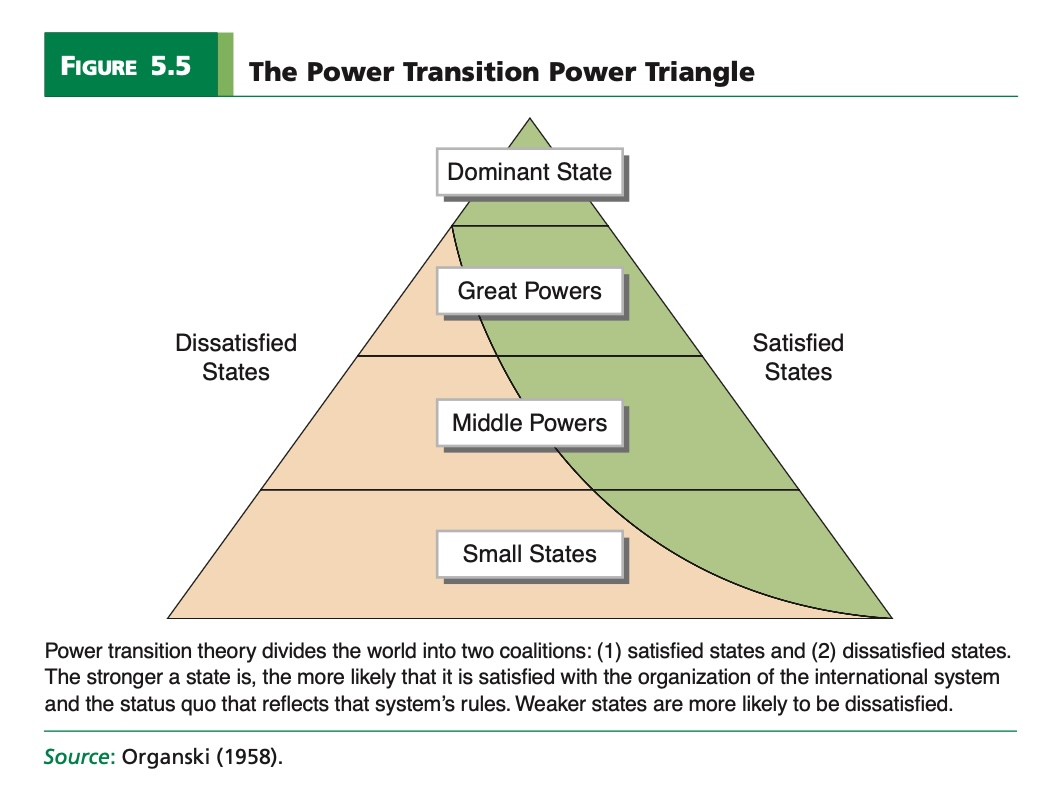
\includegraphics[width=1\textwidth]{images/power_transition_triangle.jpg}
    \captionof{figure}{\label{fig:fig1_power_transition_triangle}%\textit{\parencite[Fig.\(\backsim\)1]{cranmerWhatCanWe2017}}
    }
\end{center}

\subsection{Dissatisfaction, the Status Quo, and War}
Conflict arises when a dissatisfied state grows strong enough to challenge the authority of the hegemon. Because such a challenge concerns the very way in which international affairs are conducted, the ensuing conflict is fierce and costly.

This time period during which the challenger roughly comes to equal and then surpass the dominant state in power is known as the power transition. It is the time when the threat of a major war is hypothesized to be at its peak.
\textbf{Contrary to the balance-of-power perspective}, power transition and hegemonic stability theorists believe that major wars are most likely to occur when the power of the opposed states is about equal.

\textbf{According to these theorists, a balance of power promotes war.} They maintain that system-transforming wars—that is, wars that lead to a new power hierarchy and to new rules and norms—will occur only when the power of a challenger and the dominant state are about equal and the power of the challenger is increasing faster than that of the dominant state. These claims have been extended and shown to have \textbf{empirical strength} at the regional as well as the global level, so that regional hegemons apparently face the same pressures and the same sources of war as their global counterparts.

Threatening balance of power emerges as a result of differing rates of internal growth between a dominant state and a challenger state. These theories still give little attention to domestic politics per se, but they do recognize that internal factors shape rates of growth.

Power transition theory leads to the hypothesis that system-transforming, high-cost wars are especially likely when a dissatisfied challenger state achieves approximate power parity with the dominant, status quo-defending state.

Kim and Morrow have shown that the distribution of power at which the rivals will fight depends on their willingness to take the risks of waiting. The longer the challenger waits to attack, the higher is its probability of victory. This is true because the challenger’s power is growing faster than the dominant state’s power. Thus, the longer the challenger puts off a war, the greater will be the odds in its favor. However, the longer it waits, the longer it must endure the rules of international intercourse with which it is dissatisfied.

Kim and Morrow have shown that the interval during which the challenger is willing to fight expands as the expected costs of the war increase, as the challenger’s dissatisfaction with the status quo increases, as the challenger’s relative growth rate declines, and as the challenger becomes more risk acceptant.

How long the challenger and the dominant states will wait before fighting depends on their respective responses to risk, their relative rates of growth, the expected costs of the war, and their respective degrees of satisfaction with the status quo.

Differences in growth rates turn out not to be crucial empirically.

Power transitions per se cannot explain especially costly wars.

\begin{center}
    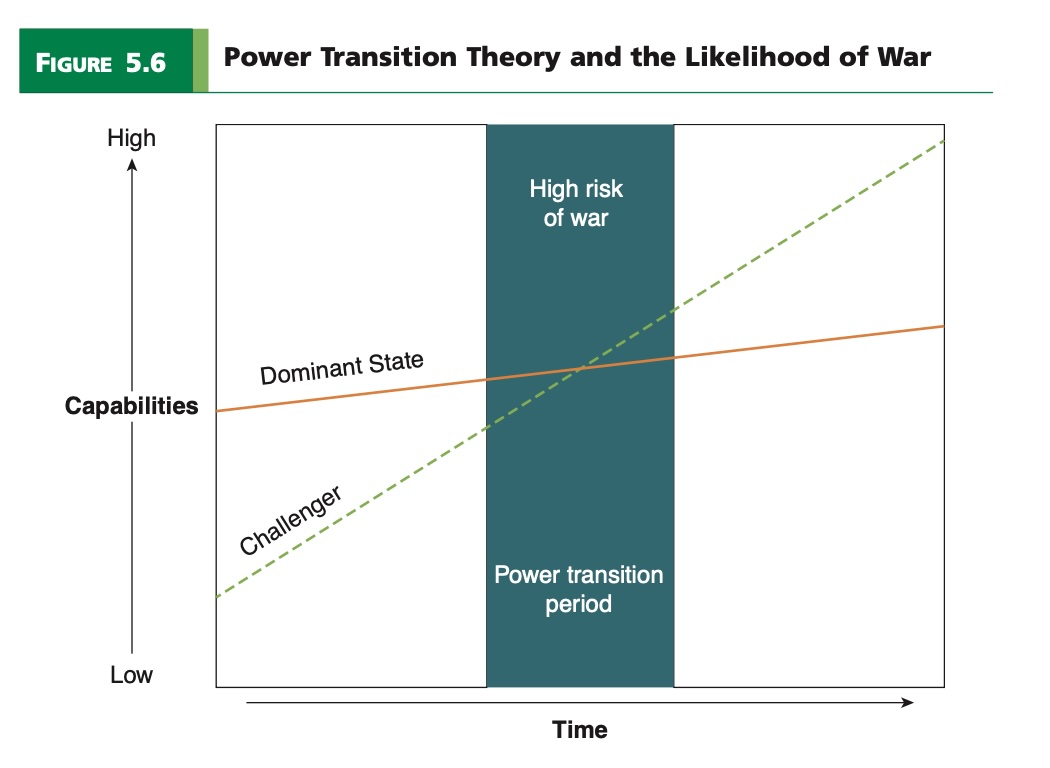
\includegraphics[width=1\textwidth]{images/power_transition_pattern.jpg}
    \captionof{figure}{\label{fig:fig1_power_transition_pattern}%\textit{\parencite[Fig.\(\backsim\)1]{cranmerWhatCanWe2017}}
    }
\end{center}

\newpage

\section{\cite{levyCAUSESWARCONDITIONS}}
This makes it hard to argue that human nature and related factors are causes of war. The point is that these factors are constants and cannot explain the variations in war and peace over time and space (Waltz 1959, Cashman 1993).

Why does war occur at some times rather than other times, between some states rather than other states, under some political leaders rather than others, in some historical and cultural contexts rather than others, and so on? This differs from still a third question: How do we explain the origins of a particular war? Most international relations scholars (and particularly those in North America) focus primarily on the second question, explaining variations in war and peace. They leave the question of why war occurs at all to philosophers and biologists and leave the question of why a particular war occurs to historians.

Although \textbf{anarchy} may provide one persuasive answer to the question of the permissive causes of war, it is generally treated as a structural constant and consequently it cannot account for variations in war and peace.

\subsection{The Levels-of-Analysis Framework}
Waltz (1959) classified the causes of war in terms of their origins in the individual, the nation-state, and the international system $\Rightarrow$ levels-of-analysis framework as an organizing device for the study of war.

In this sense the systemic level of analysis refers to explanations of patterns and outcomes in the international system; the dyadic level refers to explanations of the strategic interactions between two states; the national level refers to explanations of state foreign policy behavior; the organizational level refers to explanations of the behavior of organizations; and the individual level refers to explanations of the preferences, beliefs, or choices of individuals.

We cannot assume that correlations or causal connections at one level of analysis are necessarily valid at another level. It is conceivable, for example, that concentrations of power may promote peace at the dyadic level but war at the system level.

\subsection{Systemic-Level Theories}
The realist tradition has dominated the study of war since Thucydides and includes Machiavellians, Hobbesians, classical balance of power theorists, Waltzian neorealists, and hegemonic transition theorists. Although different realist theories often generate conflicting predictions, they share a core of common assumptions: the key actors in world politics are sovereign states that act rationally to advance their security, power, and wealth in a conflictual international system that lacks a legitimate governmental authority to regulate conflicts or enforce agreements.

\begin{itemize}
    \item they use Prisoner's Dilemma and stag-hunt models
    \item The core proposition of realist theory is that the distribution of power, throughout the system or within a dyad, is the primary factor shaping international outcomes.
\end{itemize}

We should treat realism as a paradigm rather than as a theory, and focus instead on specific theories that generate more determinant, testable propositions.

\subsubsection{Hegemonic Theory or Power Transition Theory}
Hegemonic theory is a structural theory that incorporates power transition theory and hegemonic stability theory and that \textbf{downplays the importance of anarchy}.

Hegemons commonly arise and use their strength to create a set of political and economic structures and norms of behavior that enhance the stability of the system while advancing their own security. Differential rates of growth, the costs of imperial overextension, and the development of vested domestic interests lead to the rise and fall of hegemons, and the probability of a major war is greatest at the point when the declining leader is being overtaken by the rising challenger.

Power transition theorists disagree somewhat on the precise identity of hegemonic wars and the particular causal dynamics from which they arise.

\subsubsection{Balance of Power Theory}
Balance of power theory is more concerned with explaining national strategies, the formation of blocking coalitions, the avoidance of hegemony, and the stability of the system than the origins of wars, which are underdetermined.

There is a major debate, however, between classical realists, who argue that stability is further supported by the presence of a multipolar distribution of power and a “flexible” alliance system (Morgenthau 1967, Gulick 1955), and neorealists, who argue that bipolarity is more stable than multipolarity (Waltz 1979, Mearsheimer 1990).

\textbf{Balance of power theory and power transition theory appear to be diametrically opposed}; the former argues that hegemony never occurs and that concentrations of power are destabilizing, and the latter argues the opposite.

\subsubsection{Realism and Liberalism}
The relationship between economic interdependence and war is an old question that has attracted new attention in the past few years.

\textbf{Liberal economic theory of war:} Montesquieu [1977 (1748)] stated that “peace is the natural effect of trade,” and liberal economic theorists since Smith [1937 (1776)] and Ricardo [1977 (1817)] have argued that capitalist economic systems and the free exchange of goods in an international market economy are the best guarantors of peace.

\textbf{Realist:} they often argue that the effect of trade on war is small relative to that of military and diplomatic considerations. They also question the liberal assumption that trade is always more efficient than military coercion in expanding markets and investment opportunities and in promoting state wealth.

Whether the incentives for the gains from trade dominate the incentives for coercion or protection based on economic asymmetries, and whether the latter escalate to trade wars and militarized conflicts, are empirical questions that analysts have only recently begun to analyze systematically.

\textbf{Historical and empirical evidence of trade between enemies}

Although liberals and realists disagree on the effects of trade on war, \textbf{they appear to agree that trade and other forms of economic interchange between societies will cease or be drastically reduced once states are at war with each other.} Contrary to both liberal and realist expectations, however, \textbf{there are numerous historical cases of trade between enemies} during wartime, and a preliminary quantitative study suggests that war frequently does little to depress the volume of trade between adversaries (Barbieri \& Levy 1997).

Need to incorporate domestic variables into their hypotheses

\textbf{States often hesitate to terminate trade with the enemy for fear that they will lose that trade to a third party}, who may be a greater economic or military rival.

These omissions have led all but the most committed neorealists to conclude that \textbf{systemic-level theories are theoretically incomplete and empirically inadequate}, in that \textbf{they leave too much of the variation in the outbreak and expansion of war unexplained.}
